\documentclass{article}

% if you need to pass options to natbib, use, e.g.:
% \PassOptionsToPackage{numbers, compress}{natbib}
% before loading nips_2017
%
% to avoid loading the natbib package, add option nonatbib:
% \usepackage[nonatbib]{nips_2017}

\usepackage{graphicx}
\usepackage{amsmath}
\usepackage{float}
\usepackage{bm}
\usepackage{bbm}

\graphicspath{ {../figs/}}

\usepackage[final]{report}

% to compile a camera-ready version, add the [final] option, e.g.:
% \usepackage[final]{nips_2017}

\usepackage[utf8]{inputenc} % allow utf-8 input
\usepackage[T1]{fontenc}    % use 8-bit T1 fonts
\usepackage{hyperref}       % hyperlinks
\usepackage{url}            % simple URL typesetting
\usepackage{booktabs}       % professional-quality tables
\usepackage{amsfonts}       % blackboard math symbols
\usepackage{nicefrac}       % compact symbols for 1/2, etc.
\usepackage{microtype}      % microtypography

\DeclareMathOperator*{\argmax}{arg\,max} % thin space, limits underneath in displays

\title{Gaussian process classifiers for CNN uncertainty}

% The \author macro works with any number of authors. There are two
% commands used to separate the names and addresses of multiple
% authors: \And and \AND.
%
% Using \And between authors leaves it to LaTeX to determine where to
% break the lines. Using \AND forces a line break at that point. So,
% if LaTeX puts 3 of 4 authors names on the first line, and the last
% on the second line, try using \AND instead of \And before the third
% author name.

\author{
  Sebastian Borgeaud dit Avocat \\
  LE49 - Probabilistic Machine Learning Project
  }

\begin{document}
%\nipsfinalcopy is no longer used

\maketitle

\begin{abstract}
Gaussian processes can be used in conjunction with neural networks to obtain prediction uncertainty bounds without decreasing performance. In this project, I focus on the MNIST dataset and show how uncertainty bounds can be obtained using a CNN. Furthermore, I inspect how these uncertainty bounds increase when presented with input data coming from a different underlying distribution than the training data. Finally, I show how the uncertainty bounds can be incorporated into the model to give the model the option to reject classifying examples for which it is too uncertain and evaluate this model using a metric that weighs misclassification and classification rejection according to user-defined weights.
\end{abstract}

\section{Introduction}
Model uncertainty is of crucial importance in many regression and classification tasks such as medical diagnosis, autonomous vehicle steering or high frequency trading \cite{Gal2016Uncertainty}. With model uncertainty it is possible to treat uncertain inputs and special cases explicitly. For example, if model uncertainty is high, a human expert could be asked to decide whether a particular MRI scan shows signs of a tumour or not. Another example showing how model uncertainty could be utilised is when the model is allowed to reject classifying certain examples. In this case the model could reject classification for those examples for which it is too uncertain.

Although deep learning models have become the state-of-the-art in many of those tasks, they do not capture model uncertainty \cite{gal2016dropout}. In classification tasks, the last layer is often passed through a softmax activation which returns a probability distribution over the classes \cite{Goodfellow-et-al-2016}. However, a high probability doesn't mean that the model is certain of its prediction: the model could give a high probability with a high uncertainty in which case the prediction might be worthless \cite{gal2016dropout}.

Finding ways to integrate Bayesian uncertainty with deep learning models has become a hot research topic. For example, Yarin Gal shows how dropout in neural networks can be used to obtain uncertainty bounds \cite{gal2016dropout}. In this project, I present one method to obtain uncertainty bounds for convolutional neural networks: using a Gaussian process on the last-layer features learned by the CNN. In particular, I focus on the task of classifying hand-written digits using the MNIST dataset \cite{lecun1998gradient}.

\section{Background}
\subsection{Convolutional neural networks}
Convolutional neural networks (CNNs) have become standard in many deep learning applications, especially in image processing or vision tasks \cite{Goodfellow-et-al-2016}. A convolutional neural network is a type of feedforward neural network, typically consisting of convolutional layers, pooling layers and fully connected layers \cite{DBLP:journals/corr/GuWKMSSLWW15}:
\begin{itemize}
	\item \textbf{Convolutional layers} are composed of  several 	convolution kernels each computing a different feature map. The output feature maps are obtained by convolving the input with the convolution kernel and then applying an element-wise nonlinearity. Mathematically, the feature value $z_{i,j,k}^l$ at location $(i,j)$ of the $k\textsuperscript{th}$ feature map in the $l\textsuperscript{th}$ layer is computed as:
	\[z_{i,j,k}^l = {\mathbf{w}_k^l}^T \mathbf{x}_{i,j}^l + b_k^l\]
	where  $\mathbf{w}_k^l$ and $b_k^l$ are the weight and bias vectors for the $k\textsuperscript{th}$ convolution kernel in the $l\textsuperscript{th}$ layer and $\mathbf{x}_{i,j}^l$ is the input patch centered around $(i,j)$ in the $l\textsuperscript{th}$ layer. The ouput value is computed by apply a nonlinearity $a(\cdot)$ point-wise:
	\[x_{i,j,k}^{(l+1)} = a(z_{i,j,k}^l) \]

	\item \textbf{Pooling layers} aim to achieve shift-invariance and reduce the number of parameters in the network by reducing the resolution of the feature maps. The pooling layer operates on each feature map independently. Mathematically, the output of a pooling layer with pooling operation $\textrm{pool}(\cdot)$ is given by 
	\[ y_{i,j,k}^l = \textrm{pool}(x^l_{m,n,k}), \forall (m,n) \in \mathcal{R}_{i,j}\]
	where $\mathcal{R}_{i,j}$ is a local neighbourhood around $(i,j)$. Typically, the pooling operation computes the average or the maximum.
	
	\item \textbf{Fully connected layers} connect every neuron in the previous layer to every neuron in the current layer. Mathematically, the output of a fully connected layer is given by:
	\[ x^{(l+1)}_i = a\Big(\big( \sum_j w_{i,j}^l x^l_j \big) + b^l_i\big)\]
	where $a(\cdot)$ is a nonlinearity, $w_{i,j}^l$ is the weight connecting neuron $j$ in the $l\textsuperscript{th}$ layer to neuron $i$ in layer $(l+1)\textsuperscript{th}$, and $b_i^l$ is the bias weight for neuron $i$.
\end{itemize}
The learning process for convolutional neural network is identical to the learning process for standard neural networks. A differentiable loss function is computed for the training examples (often done in batches) and the gradients w.r.t.\ the weights of the network are computed. Using these gradients, the weights are updated in a gradient descent step. Typically, more complex update rules that take into account momentum (e.g. Adam optimisation \cite{adam}) are used as they converge faster. 

\subsection{Gaussian processes}
Formally, a Gaussian Process is defined as a collection of random variables, any finite number of which have (consistent) joint Gaussian distributions. A Gaussian process therefore defines a distribution over functions and is fully specified by a mean function $m(x)$ and a covariance function $k(x, x')$. Write $f \sim \mathcal{GP}(m, k)$ meaning $f$ is distributed as a GP with mean $m$ and covariance $k$.

Using the GP we can draw samples from the function for any finite number $n$ of locations. Given locations $\mathbf{x} = [x_1, \dots, x_n]$, first compute $\mu_i = m(x_i)$, $\Sigma_{i,j} = k(x_i, x_j)$. We can then sample a vector from this distribution: $\mathbf{f} \sim \mathcal{N}(\mathbf{\mu}, \mathbf{\Sigma})$.

\subsubsection{Regression}
We can now use this GP as a prior for Bayesian inference. Let $\mathbf{f}$ be the known function values for the training examples an let $\mathbf{f}_*$ be the set of function values corresponding to the set of test inputs $X_*$. The joint distribution is given by
\begin{equation*}
\begin{bmatrix} \mathbf{f} \\ \mathbf{f}_* \end{bmatrix} 
= 
\mathcal{N}\Big(\begin{bmatrix} \bm{\mu} \\ \bm{\mu}_* \end{bmatrix}, \begin{bmatrix}\bm{\Sigma} & \bm{\Sigma}_* \\ \bm{\Sigma}_*^T & \bm{\Sigma}_{**} \end{bmatrix} \Big)
\end{equation*}
where $\bm{\mu}_*$ are the test means, $\bm{\Sigma}_*$ are the training-test covariances, and $\bm{\Sigma}_{**}$ are the test-test covariances. Since we know the training values $\mathbf{f}$, we are interested in the conditional distribution of $\mathbf{f}_*$ given $\mathbf{f}$:
\begin{equation*}
	\mathbf{f} \big\vert \mathbf{f}_* \sim
	\mathcal{N} \big( \bm{\mu}_* + \mathbf{\Sigma}_*^T \mathbf{\Sigma}^{-1}(\mathbf{f}-\bm{\mu}), \mathbf{\Sigma}_{**} - \mathbf{\Sigma}^T_*\mathbf{\Sigma}^{-1}\mathbf{\Sigma}_* \big)
\end{equation*}
This corresponds to a posterior Gaussian process $f \big\vert \mathcal{D} \sim \mathcal{GP}(m_\mathcal{D}, k_\mathcal{D})$, where
\begin{align*}
	 m_\mathcal{D}(x) = m(x) + \Sigma(X,x)^T\Sigma^{-1}(\mathbf{f}-\mathbf{m})\\
	k_\mathcal{D}(x, x') = k(x, x') - \Sigma(X,x)^T\Sigma^{-1}\Sigma(X, x')
\end{align*}
where $\Sigma(X, x)$ is a vector of covariances between every training case in $X$ and x. Furthermore, it is easy to incorporate noise in the observations. Assuming i.i.d.\ additive Gaussian noise, every $f(x)$ now has extra covariance with itself with a magnitude equal to the noise variance $\sigma_n^2$:
\begin{equation*}
	f \big\vert \mathcal{D} \sim \mathcal{GP}(m_\mathcal{D}, k_\mathcal{D} + \delta_{ii} \sigma_n^2)
\end{equation*}
where $\delta_{ii'} = 1$ iff $i=i'$ is the Kronecker's delta.

The mean function $m(x)$ and the covariance function $k(x,x')$ are typically parametrised in terms of hyper-parameters $\bm{\theta}$. During training we find the values of the hyper-parameters which optimise the marginal likelihood:
\begin{equation*}
	L = \log p(\bm{y}\vert\bm{x},\bm{\theta}) = -\frac{1}{2}\vert\Sigma\vert - \frac{1}{2}(\bm{y}-\bm{\mu})^T\Sigma^{-1}(\bm{y}-\bm{\mu}) - \frac{n}{2}\log(2\pi)
\end{equation*}
This optimisation can be done using standard gradient methods.
\subsubsection{Classification}
\paragraph{Binary classification} using Gaussian processes can be done by setting a GP prior over a latent function $f(\mathbf{x})$ and then using squashing function such as the sigmoid to obtain a probability:
\begin{equation*}
	\pi(\mathbf{x}) = p(y = +1 \vert \mathbf{x}) = \sigma(f(\mathbf{x}))
\end{equation*}
Inference is done in two steps. First, the distribution of the latent variable corresponding to a new test input $\mathbf{x}_*$ is computed:
\begin{equation*}
	p(f_*  \vert \mathbf{X}, \mathbf{y}, \mathbf{x}_*) = \int p (f_*  \vert \mathbf{X}, \mathbf{x}_*, \mathbf{f}) p(\mathbf{f} \vert \mathbf{X}, \mathbf{y}) d\mathbf{f}.
\end{equation*}
Second, a probabilistic prediction is computed using the distribution computed in the first step:
\begin{equation*}
	\bar{\pi}_* = p(y_* = +1 |\mathbf{X}, \mathbf{y}, \mathbf{x}_*) = \int \sigma(f_*) p(f_*  \vert \mathbf{X}, \mathbf{y}, \mathbf{x}_*) df_*
\end{equation*}
As the likelihood is non longer Gaussian, the first integral becomes analytically intractable. Similarly, depending on the sigmoid function, the second integral can also be intractable. Hence, we need to use approximations, either analytical or numerical, for example using Monte Carlo sampling, to solve the integrals.


\paragraph{Multi-class classification} is typically \cite{villacampa2017scalable} approached by assuming the following labelling rule for $y_*$ given $\mathbf{x}_*$:
\begin{equation*}
	y_* = \argmax_{k=1,\dots,C} f^k(\mathbf{x}_*)
\end{equation*} 
where each $f^k(\cdot)$ is a nonlinear latent function with a GP prior and $C$ is the number of classes. The likelihood is again non-Gaussian meaning that approximation techniques have to be used to perform inference and to optimise the hyper-parameters.

\subsection{Uncertainty in Deep Learning}
Current deep learning methods only give point estimates of parameters and predictions \cite{Goodfellow-et-al-2016}. Despite the fact the output of a softmax layer in a classification task can be interpreted as a probability distribution $p(y_i = k) = f(x_i)_k$, the probabilities say nothing about how certain the model is: The model could assign a high probability to a class but can still be highly uncertain about it \cite{gal2016dropout}. 

One way to obtain uncertainty bounds from deep learning models was discovered by Yarin Gal. In fact, Gal \cite{Gal2016Uncertainty} showed that dropout training in neural networks can be casted as approximate Bayesian inference in deep Gaussian processes. In particular, he showed that using Dropout not only at training time but also at test time gives a principled way of computing uncertainty bounds by sampling multiple estimates from the model and computing their sample variance \cite{Gal2016Uncertainty}.

In this project, I focus on a different way to obtain those uncertainty bounds: Using a Gaussian process trained on the features extracted by a CNN that was trained in a previous step on the same test training data. It should be noted that this is a less theoretically grounded approach than the one taking by Gal, but nonetheless provides a practical way of getting uncertainty bounds without losing the power of deep learning models. 

\section{Method}
\subsection{Convolutional Neural Network architecture}
The first step consists of training the convolutional neural network, which can be done using one of the many deep learning libraries. For example, I use Keras \cite{chollet2015keras} which defines an extra abstraction layer above TensorFlow. The network architecture is provided in the Keras tutorial for image classifcation on MNIST. The first two layers are convolutional layers with $3 \times 3$ kernels and ReLU activations, where $\textrm{ReLU}(x) = \max(x, 0)$. These layers have respectively 32 and 64 feature maps. A max-pooling layer with kernel size $2 \times 2$ is then applied to the output of the convolutional layer. The final 2 layers are fully connected layers consisting of 128 and 10 neurons respectively. The first fully connected layer has a ReLU activation. The last fully connected layer uses a softmax activation, which outputs a probability distribution over the 10 classes representing the 10 digits. Furthermore, Dropout \cite{srivastava2014dropout} is applied after the max-pooling layer with $p=0.25$ and after the first fully connected layer with $p=0.5$, where $p$ is the probability of dropping a neuron. The network is trained using an Adadelta optimiser over 10 epochs with batches of size 128.

\subsection{Training of the Gaussian process}
From the trained CNN model, the activations of the last hidden layer are extracted. These correspond to a vector of size 128 for each input image, and can be thought of as the features extracted by the CNN for classification. Using these features I then train a Gaussian Process. This has the advantage of being a lower dimensional classification task compared to classifying the entire input image directly, whilst still being fully automatic, i.e.\ there are no user-defined features. However, the MNIST dataset, with 60,000 training images, is considered a large dataset for GPs because inference takes $\mathcal{O}(n^3)$ time where $n$ is the number of training instances \cite{hensman2015scalable}. To make the training possible, I use GPFlow \cite{GPflow2017}, which implements various approximation algorithms for Gaussian Processes. Furthermore, the library is built on top of TensorFlow which has the further advantage of being usable on a GPU out-of-the-box, which provides a further speed-up. More precisely, I use the Sparse Variational Gaussian Process Classifier presented by Hensman et al.\ \cite{hensman2015scalable}. The model learns a set of m inducing points which are used instead of the training points in the Gaussian process. Typically, $m < n$, which makes the task tractable as its complexity is $\mathcal{O}(nm^2)$. For the experiments done in this project I chose to use 600 inducing points, which allowed the model to be trained in about 15 minutes on a NVidia Titan Xp GPU.

I train the Gaussian process with a simple kernel as it is sufficient to obtain good accuracy. The kernel consists of a Matern kernel  \cite{rasmussen2006gaussian} with $\nu =\frac{3}{2}$ and a white noise function to account for the noise in the input data.

\subsection{Classifying with a reject option}
\label{section/reject_option}
One way to incorporate the model uncertainty is by allowing the model to say ``I don't know''. For example, if the model was presented with an image of the letter `a', it would still classify the image into one of the 10 digits, which might not be a desired outcome. Instead, the model should be able to reject classification for the inputs in which the uncertainty is too high. This is known as \textbf{classification with a reject option} \cite{chow1970optimum}. 

Given uncertainty bounds with each class probability, we can design the model to reject classification according to certain rejection rules. We could decided to reject if the standard deviation of the highest probability is above a pre-defined threshold. Another rejection rule could be to reject if the second highest class probability lies within a certain factor $\epsilon$ of the standard deviations of the highest probability, i.e.\ the model would reject if
\begin{equation*}
	\vert f_p(\mathbf{x}^{(i)})_1 - f_p(\mathbf{x}^{(i)})_2 \vert < \epsilon f_{\textrm{std}}(\mathbf{x}^{(i)})_1
\end{equation*}
where $f_p(\mathbf{x}^{(i)})$ is the classification probability vector for input $\mathbf{x}^{(i)}$ with $f_p(\mathbf{x}^{(i)})_j$ being defined as the probability of the $j\textsuperscript{th}$ most likely class, and $f_{\textrm{std}}(\mathbf{x}^{(i)})_1$ is the standard deviation of the most likely class returned by the model for input $\mathbf{x}^{(i)}$. Note that the $\epsilon$ parameter defines a trade-off between the number of misclassified examples at the number of examples that would have been correctly classified but were rejected instead.

\subsection{Evaluation}
\subsubsection{Accuracy}
The standard metric for evaluating a model $f$ on a classification task is the accuracy: 
\begin{equation*}
	\textrm{accuracy} = \frac{1}{N} \sum_{i=1}^N \mathbbm{1}(f(\mathbf{x}^{(i)}) = y^{(i)})
\end{equation*}
where $N$ is the number of test data points and $(\mathbf{x}^{(i)}, y^{(i)})$ is the $i\textsuperscript{th}$ test point. Note that the accuracy does not take into account the uncertainty with which a model makes the prediction and only rewards correctly classified examples.

\subsubsection{R-accuracy}
 An appropriate metric for classification with a reject option assigns a cost $\alpha$ to misclassification and a cost $\beta$ to the reject option \textregistered:
\begin{equation*}
	\textrm{R-accuracy}_{\alpha, \beta} = \frac{1}{N} \sum_{i=1}^N \mathbbm{1}(f(\mathbf{x}^{(i)}) = y^{(i)}) - \alpha \mathbbm{1}(f(\mathbf{x}^{(i)}) \neq y^{(i)}) - \beta \mathbbm{1}(f(\mathbf{x}^{(i)}) = \textregistered)
\end{equation*}
Here, $\alpha$ and $\beta$ are parameters that are set by the user. A large value for $\alpha$ corresponds to cases where misclassification is expensive, for example in medical diagnosis or when a self-driving car has to make a steering decision. The $\beta$ parameter intuitively indicates how much value the user places on obtaining a prediction, as a higher $\beta$ will increase the cost of the reject option.

\section{Results}
\subsection{MNIST dataset}
The MNIST dataset is considered a toy dataset in deep learning. In fact, using the model described above, I obtain an accuracy of $99.12\%$ on the held-out test images. This means that only $88$ of the $10,000$ test images are misclassified.

Using the Gaussian process with the CNN features, the accuracy of the model on the test images improves to $99.28\%$, reducing the number of misclassified images to $72$. Although this increase in performance might seem surprising at first, it can be explained by the fact that the Gaussian process is more complex and more powerful than the last layer of the CNN, which just computes a linear combination of the features and then applies the softmax activation. The results obtained on the MNIST dataset are summarised in the table \ref{table/mnist_acc}.

\begin{table}[h]
\centering	
{\renewcommand{\arraystretch}{1.2} %<- modify value to suit your needs
\begin{tabular}{ c | c c}
\textbf{Model} & \textbf{Accuracy} & \textbf{Misclassified images}\\
\hline
CNN & $99.12\%$ & $88$ \\
GP & $99.28\%$  & $72$\\
\end{tabular}
}
\caption{MNIST test images accuracy for the CNN and the GP.}
\label{table/mnist_acc}
\end{table}

Furthermore, it is interesting to inspect how uncertain the Gaussian process is for the different test images. In order to do this, I plot in figure \ref{fig/mnist_cum_stds} the cumulative distribution of the standard deviations for the most likely class for both correctly and incorrectly classified test images. For the correctly classified examples, the model's uncertainty is low: the model gives the correct class probability with a standard deviation of less than $0.1$ for $97.3\%$ of the correctly classified images. However, for the incorrectly classified images, the standard deviation of the most likely class seems to be higher: The model predicts a standard deviation below $0.1$ for only $19.4\%$ of the incorrectly classified images. This suggests that the model is generally less certain of its prediction in the cases where it predicted the wrong class.
\begin{figure}
	\centering
	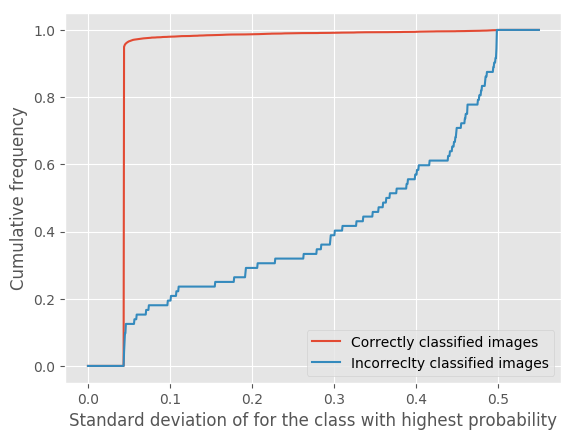
\includegraphics[scale=0.3]{mnist_cum_stds}
	\caption{Cumulative distribution of the standard deviations for the most likely class for both correctly and incorrectly classified test images.}
	\label{fig/mnist_cum_stds}
\end{figure}

\subsection{Noisy MNIST (n-MNIST)}
I evaluate both the CNN and the Gaussian process on the n-MNIST dataset \cite{DBLP:journals/corr/BasuKGDMN15}. The dataset consists of the MNIST images, but modified in 3 different ways so as to make the classification task harder. The first set of images is created by adding white Gaussian noise with a signal-to-noise ratio of 9.5 to the images. The second set of images is obtained by emulating a linear motion blur. The last set of images is the hardest to classify as it is created by reducing the contrast and also adding white Gaussian noise to the original images. Figure \ref{fig/noisy_mnist_example} shows an example image taken from the 3 datasets.

\begin{figure}
	\centering
	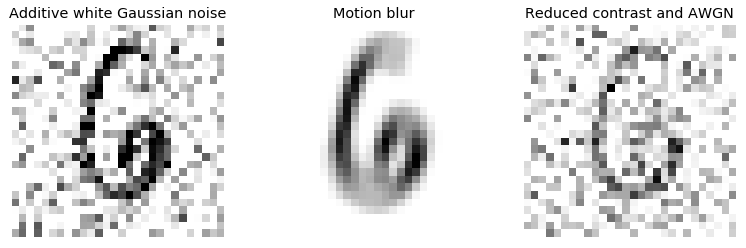
\includegraphics[scale=0.2]{noisy_mnist_example}
	\caption{Example digits from the noisy-MNIST dataset. From left to right: Additive white Gaussian noise, Motion blur, and Reduced contrast with AWGN}
	\label{fig/noisy_mnist_example}
\end{figure}

The task of classifying examples whose underlying distribution is different from the underlying distribution of the training images is called \textbf{out-of-distribution} classification \cite{Gal2016Uncertainty}. The performance of the two models is shown in table \ref{table/noisy_mnist_acc}. Although the GP performs better on the NMIST test images, the CNN performs better on all 3 noisy datasets. This could again be explained by the fact that the GP is a more complex model, therefore is overfitting more on the NMIST data and hence is not able to generalise as well on these different datatsets. Especially noticeable is the difference in performance for the reduced contrast dataset, where the CNN obtains an accuracy of $77.71\%$ compared to $70.13\%$ for the GP. As the 3\textsuperscript{rd} dataset is the least similar the original one, this higher discrepancy supports the claim that the GP is overfitting more on the MNIST dataset.

\begin{table}[h]
\centering	
{\renewcommand{\arraystretch}{1.2} %<- modify value to suit your needs
\begin{tabular}{ c | c c c}
\textbf{Model} & \multicolumn{3}{c}{\textbf{Accuracy}}\\
& AWGN & Motion blur & Reduced contrast\\
\hline
CNN & $94.35\%$ & $93.27\%$ & $77.71\%$ \\
GP & $93.34\%$  & $92.09\%$ & $70.13\%$ \\
\end{tabular}
}
\caption{MNIST test images accuracy for the CNN and the GP.}
\label{table/noisy_mnist_acc}
\end{table}

We can again inspect how uncertain the model is when classifying the noisy dataset by plotting the cumulative distributions of the standard deviations of the most likely digit. Figure \ref{fig/noisy_mnist_cum_stds} shows the resulting plots for each dataset, which indeed suggest that the uncertainty increases as the model is asked to classify images that are increasingly different from those it was trained on. The uncertainty for the additive white Gaussian noise dataset is higher than the uncertainty for the MNIST test dataset. This is shown by the fact that the cumulative distribution for the correctly classified images in the AWGN images is lower. Similarly, the cumulative distribution further decreases for the motion blur and reduced contrast images, with a lower classification accuracy corresponding to a higher uncertainty.

\begin{figure}
	\centering
	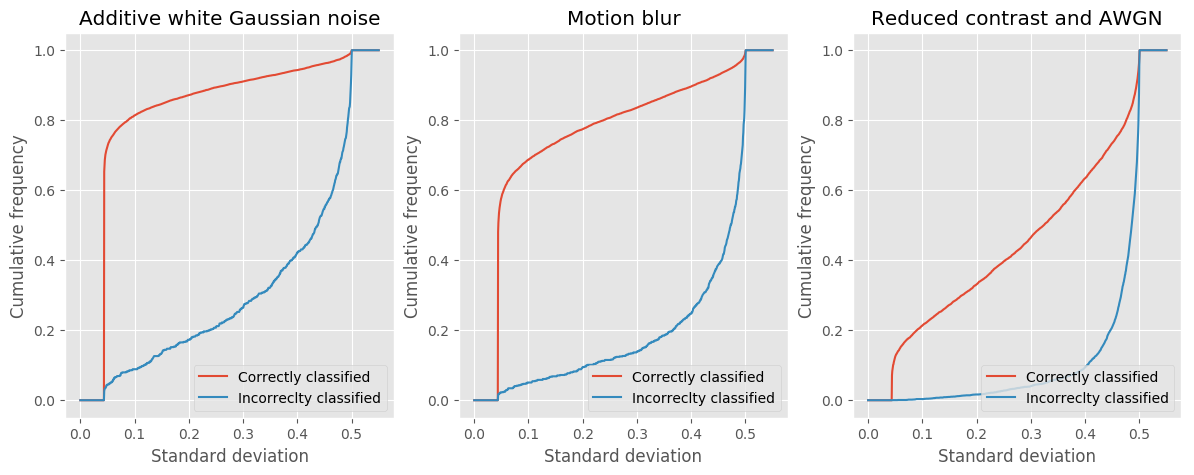
\includegraphics[scale=0.4]{noisy_mnist_cum_stds}
	\caption{Cumulative distribution of standard deviations for correctly and incorrectly classified test images on the 3 n-MNIST datasets.}
	\label{fig/noisy_mnist_cum_stds}
\end{figure}

\subsection{Classifying with a reject option}
Finally, I also evaluate the performance of the GP augmented with a reject option according to the rejection rule described in \ref{section/reject_option} on the MNIST test dataset. Figure \ref{fig/r_accs_alpha_mnist} (left) shows the R-accuracy with varying $\alpha$ and fixed $\beta=0$ for different values of $\epsilon$. In the cases where $\alpha > 1$, that is when the cost of misclassification is higher than the reward obtained by a correct classification, there seem to be an optimal value of $\epsilon$ lying between 20 and 40. 

Furthermore, there is indeed a trade-off between the number of misclassified but accepted images and the number of correctly classified but rejected images. Figure \ref{fig/r_accs_alpha_mnist} (right) illustrates this trade-off.

\begin{figure}[h]
	\centering
	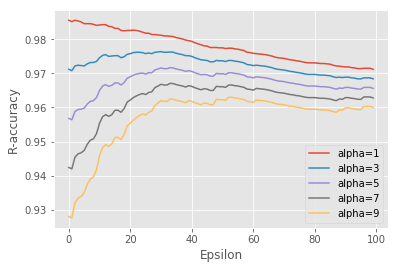
\includegraphics[scale=0.38]{r_accs_alpha_mnist}
	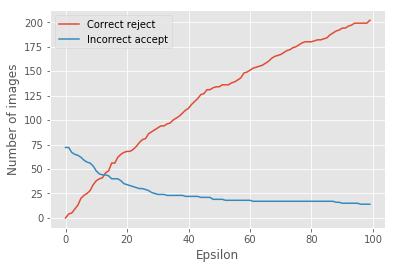
\includegraphics[scale=0.38]{r_acc_mnist}
	\caption{Left: R-accuracy obtained using varying $\epsilon$ and $\alpha$ but setting $\beta=0$. For $\alpha>0$ there seems to be an optimal value of $\epsilon$ around 30. Right: Number of examples misclassified or rejected. This illustrates the trade-off between the number of misclassified but accepted and correctly classified but rejected examples.}
	\label{fig/r_accs_alpha_mnist}
\end{figure}

\section{Discussion}
Only 72 of the 10,000 MNIST test images are misclassified by the GP. To gain some insights into why only those were misclassified, the 72 misclassified input images are shown in figure \ref{fig/incorrect_mnist} in appendix \ref{appendix/mnist_error}. The images reveal that many of those 72 images are indeed very ambiguous, even for a human annotator. For example, it is hard to say whether the first image should be a `1' or a `2'. This also explains why the uncertainty given by the model is higher for the misclassified images than it is for the correctly classified images. In fact, one could argue that for those ambiguous images the model should indeed be less certain of its prediction.

\subsection{Uncertainty with additive white noise}
A further property the model uncertainty should obey is that as an image becomes more and more distorted, the uncertainty should increase. To verify that this holds I add increasingly more white Gaussian noise to a test digit and then ask the GP to make predictions for those images. The results are shown in figure \ref{fig/awgn_predictions} for an image of the digit `6'.
\begin{figure}
	\centering
	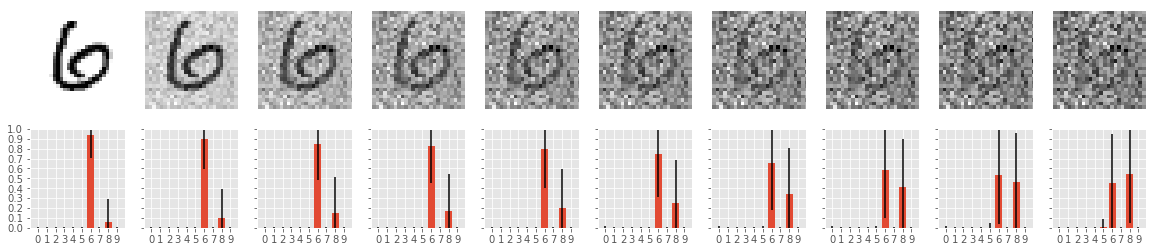
\includegraphics[width=1.0\textwidth]{awgn_predictions}
	\caption{Top: Test images with increasingly more additive white Gaussian noise. Bottom: Gausssian process predictions for the test images. The error bars show the standard error for each class.}
	\label{fig/awgn_predictions}
\end{figure}
Note that for the last few images, it becomes almost impossible to discern the original digit from the noise (especially when looked at individually, rather than next to the original image). Indeed, the model wrongly classifies the last image as a `5', although it does so with a high uncertainty. Figure \ref{fig/awgn_predictions_stds} shows the probability and uncertainty assigned to the digit `6' for the 10 images. As hoped for, the uncertainty increases as more noise is added to the image. Especially noteworthy is the increase of the standard deviation relative to the class probability.
\begin{figure}
	\centering
	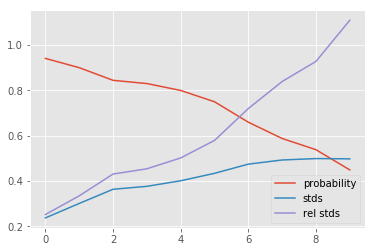
\includegraphics[scale=0.4]{awgn_predictions_stds}
	\caption{Probability and standard deviation assigned to class `6' for the 10 images shown in figure \ref{fig/awgn_predictions}. Also plotted is the standard deviation relative to the class proability.}
	\label{fig/awgn_predictions_stds}
\end{figure}

\subsection{CNN features visualisation}
Finally, I show the features learned by the CNN by reducing the number of dimensions of the features to 2 using the t-SNE \cite{maaten2008visualizing} dimensionality reduction technique. The learned features are shown for the MNIST test dataset and for the additive white Gaussian noise images of the n-MNIST dataset. Both plots show distinct clusters for the 10 different classes, but the clusters for the n-MNIST dataset seem to be less distinct. This can be explained by the fact that the network was trained on the MNIST dataset rather than on the n-MNIST dataset.

\begin{figure}
	\centering
	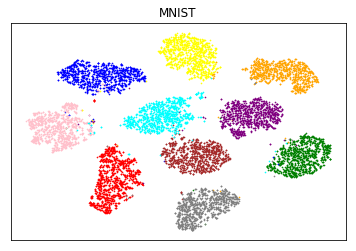
\includegraphics[scale=0.48]{embeddings_visualisation.png}
	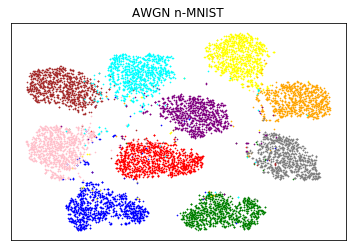
\includegraphics[scale=0.48]{noisy_embeddings_visualisation}
	\caption{Learned features for the MNIST test dataset and the AWGN n-MNIST test dataset. The dimensionality of the features were reduced using t-SNE.}
\end{figure}

\section{Conclusion}
In this project, I focused on obtaining uncertainty bounds for the MNIST and n-MNIST dataset by combining a CNN with a Gaussian process and analysed these uncertainty bounds. I showed that the uncertainty bounds given by the GP increase when presented with input data coming from a different underlying distribution than the training data. I also presented a way to add a reject option to the model by using the uncertainty bounds and letting the model reject classification for the example for which it is too uncertain. I evaluated this model using a custom metric, the R-accuracy and showed how different hyper-parameters of the metric and model affect the results. Finally, I inspected how the uncertainty bounds increase when the model is presented with increasingly more perturbed images.

\small

\bibliography{bib}
\bibliographystyle{unsrt}

\newpage
\appendix 
\section{Misclassified MNIST images by the Gaussian process model}
\label{appendix/mnist_error}

\begin{figure}[h]
	\centering
	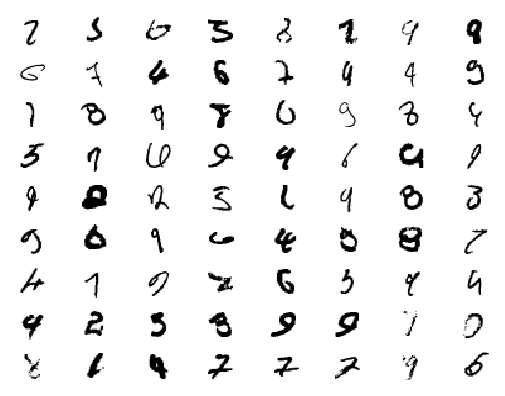
\includegraphics[scale=1.1]{incorrect_mnist}
	\caption{Test images misclassified images by the GP model.}
	\label{fig/incorrect_mnist}
\end{figure}

\end{document}
